
\section{系统原型实现}

\subsection{系统架构与技术选型}

本系统以 Python 为核心实现语言，运行环境为本地单机（Python 3.x + Conda 虚拟环境），整体采用"LLM 代理 + 传统 Python 库"的混合架构。上层通过 LangGraph\cite{langgraph2024} 组织多智能体状态机流程，下层则由 pandas、NetworkX 等库完成具体的数据处理与图计算。LangGraph 提供显式的节点—边定义和有向图执行模型，便于将第三章提出的 DAG 蓝图和多智能体分工直接映射为可执行的工程状态机。

在模型选型上，系统采用"双模型分工"策略：通义千问（Qwen）负责规划和评审，Claude 负责代码生成和执行修复。该组合的工程出发点是将"文本规划稳定性"和"代码生成能力"分开优化，降低单模型在全流程任务中的能力短板\cite{zhao2024llm,brown2020language}。具体做法上，Strategist、Methodologist 与 Reviewer 的提示词均针对 Qwen 调优，强调长文本理解、结构化输出和批判性评估；CodingAgent 的提示词则针对 Claude 调优，强调类型约束、异常处理和最小可复现单元。通过在架构层明确职责边界，可以在不改动代码框架的前提下替换底层大模型，实现平滑升级。

系统主模块代码路径如下。工作流编排在 \texttt{src/core/\allowbreak workflow.py}，规划模块在 \texttt{src/agents/\allowbreak strategist.py}（约 1520 行），方法规格化模块在 \texttt{src/agents/\allowbreak methodologist.py}，执行模块在 \texttt{src/agents/\allowbreak coding\_agent\_v4\_2.py}，评审模块在 \texttt{src/agents/\allowbreak reviewer.py}。数据感知由 \texttt{src/utils/\allowbreak data\_preview.py}（602 行）与 \texttt{src/utils/\allowbreak graph\_preview.py}（451 行）提供，知识约束由 \texttt{src/graphs/\allowbreak causal\_graph\_query.py} 与 \texttt{src/graphs/\allowbreak method\_graph\_query.py} 提供。各模块之间通过 JSON 或 Python 字典进行解耦传递，使得任何一个模块都可以在保持接口不变的前提下独立重构。

从工程职责角度，系统采用"规划—规格—执行—评审"四段式流水线，每段均有结构化 JSON 输入输出（整体架构参见图 \ref{fig:3-1}）。该方法使系统不仅能产出结果，也能产出中间证据链，便于复核与追踪\cite{hong2024metagpt,langgraph2024}。同时，结合前一章提出的三层基础能力结构，系统在流水线两端分别插入 DataPreview/GraphPreview 的数据感知模块与差距分析模块，将"数据事实—规划蓝图—执行结果"连接为闭环，有利于后续在日志与监控层面实现细粒度的错误诊断与性能分析。

\subsection{系统核心模块实现}

DataPreview 的目标是将"数据事实"前置到方案规划阶段。模块输入为 pandas DataFrame，输出为结构化预览对象，包含列类型画像、基础统计、跨列统计和抽样摘要四部分。

\subsubsection{列语义识别与类型画像}

列语义识别与类型画像是数据感知模块的入口环节，其目标是将原始数据表中“面向存储的列名”转化为“面向分析的语义标签”。系统首先识别数值列、分类列、日期列和文本列，并为每列生成质量摘要（缺失率、唯一值数、分布形态），为后续跨列统计和图构建提供必要前提。

在专利数据场景下，列名往往为中文短语且包含括号、下划线等符号，直接输入给 LLM 易产生歧义。为此，模块内置了一套列语义映射表，覆盖 30 余个常见专利字段，将列名映射为分析语义描述。例如：

\begin{table}[htbp]
\centering
\caption{列语义映射示例}
\label{tab:column-mapping}
\begin{tabular}{@{}ll@{}}
\toprule
原始列名 & 语义描述 \\ \midrule
被引用专利数量 & 被引用次数（数值维度，反映专利影响力） \\
IPC分类号 & 技术领域分类（多值分隔符列，可构建共现网络） \\
申请日 & 申请时间（日期维度，用于时间趋势分析） \\
发明人 & 发明人姓名（多值列，可构建合作网络） \\ \bottomrule
\end{tabular}
\end{table}

该映射表在实现上采用"规则模板 + 自适应匹配"的方式：一方面通过精确匹配和正则表达式覆盖常见字段（如"被引用专利数量（次）"与"被引用次数"归为同一语义），另一方面在找不到精确规则时回退到基于关键词的模糊匹配，并将低置信度映射显式标注在预览结果中。这样设计使得后续 LLM 在生成分析方案时能够直接理解每列的分析用途，避免因列名歧义导致的错误，同时保留人工复核和扩展映射表的空间。

\subsubsection{跨列统计关系抽取}

跨列统计是 DataPreview 的核心功能，用于自动发现数据中的变量关系线索，相当于在"列语义已对齐"的基础上，对潜在的变量间关系进行一次自动勘探。模块实现三类跨列统计：

\begin{enumerate}[(1)]
\item \textbf{数值列 Pearson 相关系数}。对所有数值列两两计算相关系数，过滤 $|r| > 0.1$ 的显著关联，按绝对值降序保留前 20 对。该步骤的作用是为后续假设生成提供"哪些变量之间存在线性关联"的定量线索，并避免把注意力浪费在相关性极弱的变量对上。
\item \textbf{分类列分组对比}。对低基数分类列（唯一值 $\leq$ 50），按 Top 5 类别分组计算核心数值列均值差异。例如，按"法律状态"分组计算"被引用专利数量"的均值差异，可以发现"授权|权利转移"状态的专利平均被引量是否高于普通授权专利。通过限制类别数和核心数值列数量，模块在保持信号代表性的同时控制输出长度，便于 LLM 在有限上下文中理解。
\item \textbf{时间趋势检测}。自动检测日期列，按年聚合计算核心数值列的年度均值趋势。该信号可用于发现被引量的时间衰减效应等，也为后续构造时间虚拟变量或分段回归提供依据。
\end{enumerate}
跨列统计的处理流程如算法 4-1 所示，整体数据流见图 4-1：

\begin{algorithm}[H]
\caption{跨列统计计算}
\KwIn{DataFrame df, 列类型画像 profile}
\KwOut{跨列统计结果 result}

numeric\_cols $\leftarrow$ 从 profile 中提取所有数值列\;
\tcp{相关系数计算}
corr\_matrix $\leftarrow$ df[numeric\_cols].corr(method='pearson')\;
pairs $\leftarrow$ 提取 $|r| > 0.1$ 的列对，按 $|r|$ 降序排列，取前 20 对\;
result.correlation\_pairs $\leftarrow$ pairs\;
\tcp{分组对比}
cat\_cols $\leftarrow$ 从 profile 中提取唯一值 $\leq$ 50 的分类列（取前 5 个）\;
core\_numeric $\leftarrow$ 排除 ID 类列的数值列（取前 3 个）\;
\ForEach{cat\_col in cat\_cols}{
    top\_cats $\leftarrow$ cat\_col 出现频率最高的 5 个类别\;
    \ForEach{num\_col in core\_numeric}{
        grouped\_means $\leftarrow$ df[cat\_col $\in$ top\_cats].groupby(cat\_col)[num\_col].mean()\;
        result.group\_comparisons.append(\{group\_by, metric, values\})\;
    }
}
\tcp{时间趋势}
date\_col $\leftarrow$ 检测含日期关键词的列\;
years $\leftarrow$ pd.to\_datetime(date\_col).dt.year\;
\ForEach{num\_col in core\_numeric}{
    yearly\_means $\leftarrow$ df.groupby(years)[num\_col].mean()\;
    result.time\_trends.append(\{metric, by\_year\})\;
}
\Return{result}\;
\end{algorithm}
% 图4-1
\begin{figure}[H]
\centering
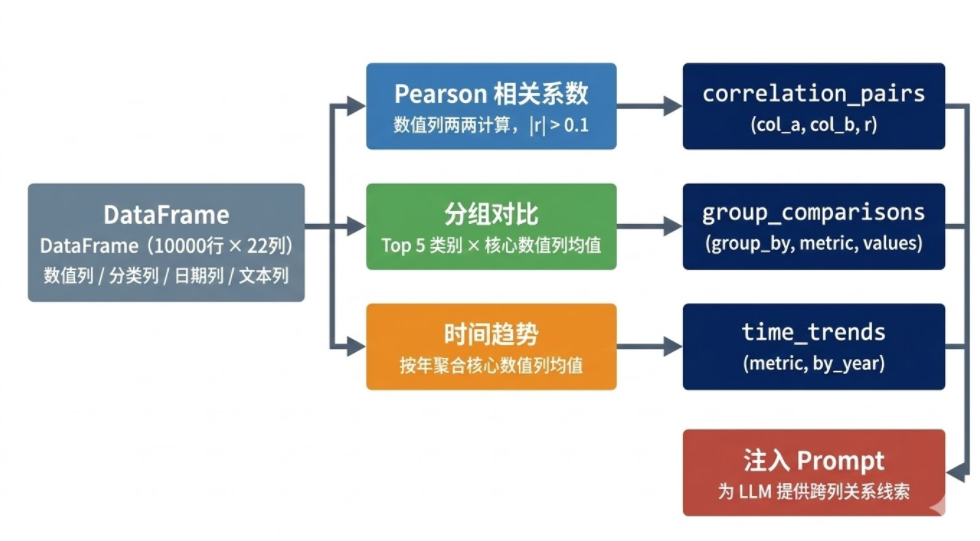
\includegraphics[width=0.95\textwidth]{figures/new_img/图4-1.png}
\caption{跨列统计数据流图}
\label{fig:4-1}
\end{figure}

\subsubsection{内容样本的分层抽样}

为让 LLM 了解专利的技术内容分布，仅依赖数值特征和 IPC 结构仍然不够，需要提供少量有代表性的摘要原文。模块按 IPC 分部（首字符 A-H）对摘要进行分层抽样，每部最多采 5 条、总计不超过 30 条，每条截断至 300 字符，使提示词在长度可控的前提下覆盖主要技术领域。

具体实现中，系统首先基于 IPC 首字符将专利划分为最多 8 个技术分部，对每个分部分别随机抽取不超过 5 条摘要；若某一分部专利数量不足 5 条，则全部纳入样本。为避免极端长摘要挤占上下文窗口，所有摘要在句子边界附近截断至约 300 字符，并保留 IPC 及基础元数据标签，便于 LLM 理解样本所属领域。

使用固定随机种子（random\_state=42）保证可复现。相比简单的全局随机抽样，分层抽样确保各技术领域均有代表性样本，降低了主题偏置，也降低了 LLM 将少数高频领域误判为总体分布的风险。

\subsubsection{图结构预览模块（GraphPreview）}

GraphPreview 用于捕捉 DataPreview 难以表达的网络结构信息，是数据感知模块中面向"关系结构"的补充维度。专利数据中存在大量多值关系字段（如 IPC 分类号、发明人、引用专利），这些字段天然可以构建为图，揭示共现关系和协作模式，从而为后续的社区发现、结构洞察和局部子网络分析提供基础。

\noindent\textbf{1.自动图构建策略}

模块首先扫描 DataFrame 中所有含分隔符的列，将其识别为"可构图候选列"。随后通过元素类型分类器判断列内元素的类型，决定构建何种图，自动构图逻辑如图 4-2 所示。

% 图4-2
\begin{figure}[H]
\centering
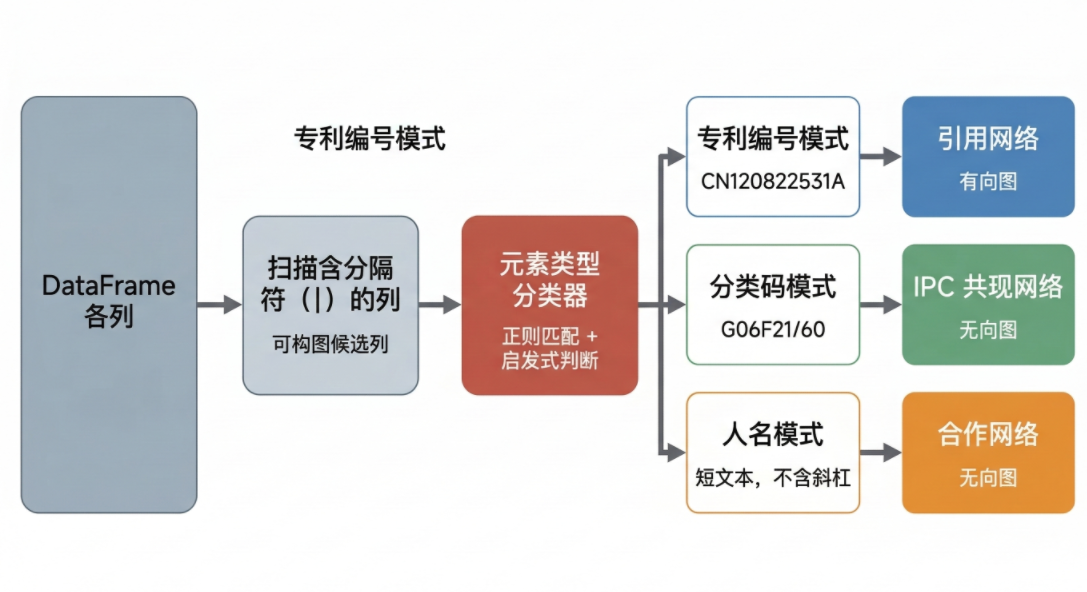
\includegraphics[width=0.95\textwidth]{figures/new_img/图4-2.png}
\caption{自动构图逻辑图}
\label{fig:4-2}
\end{figure}

分类器对采样元素进行正则匹配和启发式判断：

\begin{enumerate}[(1)]
\item 若元素匹配专利编号模式（如 CN120822531A），构建\textbf{引用网络}
\item 若元素匹配分类码模式（如 G06F21/60），构建\textbf{共现网络}
\item 若元素为短文本且不含斜杠，判定为人名，构建\textbf{合作网络}
\end{enumerate}

在实测中，系统从数据集自动构建了 6 个图：发明人合作网络、IPC 共现网络、引用网络等，无需用户显式指定"要看哪张图"。这一策略减少了使用门槛，同时保证了不同数据集在图结构分析阶段的处理流程具有可比性。

\noindent\textbf{2.分层图算法策略}

为兼顾信息密度与计算性能，模块采用分层计算策略。当图规模较小时（节点数 $\leq$ 10,000），完整计算以下指标：Louvain 社区检测（使用 python-louvain 库，固定 random\_state=42，输出社区数量、各社区规模和每社区 Top 3 代表节点）、介数中心性（对大图使用 k=500 近似采样降低复杂度，输出 Top 10 桥梁节点）、连通分量统计（输出最大连通分量占比和孤立节点数）、度分布统计（输出平均度、最大度和度分布分位数）。

当图规模超过阈值（LARGE\_GRAPH\_\allowbreak THRESHOLD = 10,000）时，跳过社区检测和介数中心性计算，仅保留度分布统计，避免 O($n^2$) 级操作导致规划阶段阻塞。这样可以在保证"大致结构特征可见"的前提下，将最耗时的运算限制在中小规模图上，对大规模数据集保持可接受的响应时间。

\begin{algorithm}[H]
\caption{图结构预览生成}
\KwIn{DataFrame df}
\KwOut{图结构指标集合 metrics}

candidate\_cols $\leftarrow$ 检测含分隔符(|)的列\;
\ForEach{col in candidate\_cols}{
    elem\_type $\leftarrow$ ClassifyElements(col) \tcp{patent\_id | classification | name}
    G $\leftarrow$ BuildGraph(col, elem\_type) \tcp{构建对应类型的图}
    \eIf{$|V(G)| > 10000$}{
        metrics[G] $\leftarrow$ \{degree\_distribution\} \tcp{仅度分布}
    }{
        communities $\leftarrow$ Louvain(G, random\_state=42)\;
        centrality $\leftarrow$ BetweennessCentrality(G, k=500)\;
        components $\leftarrow$ ConnectedComponents(G)\;
        metrics[G] $\leftarrow$ \{communities, centrality, components, degree\_distribution\}\;
    }
}
\Return{metrics}\;
\end{algorithm}

模块的关键设计原则是\textbf{只输出结构化事实，不做语义解读}。例如，输出"节点 H04L9/40 的介数中心性为 0.31"，而不输出"H04L9/40 是技术桥梁"——后者的判断由 LLM 在洞察生成阶段完成。

\subsubsection{数据洞察生成机制}

数据洞察生成是数据感知方案的核心环节，位于"数据预览"和"蓝图规划"之间，负责把前者输出的数值特征、图结构特征和摘要样本综合成面向分析的高层信号。该过程由 Strategist 中的 \path{_generate_data_insights()} 方法实现，将 DataPreview 与 GraphPreview 的输出合并为 LLM 提示词，驱动 LLM 生成结构化的可检验洞察。

\paragraph{洞察生成的 Prompt 设计}

Prompt 设计遵循"输入尽量完备、输出尽量克制"的原则，包含三层输入和严格的输出约束：

\textbf{输入层}：

\begin{enumerate}
\item 数据统计特征（来自 DataPreview 的相关系数、分组对比、时间趋势）
\item 图结构分析（来自 GraphPreview 的社区、中心性、连通分量）
\item 领域摘要样本（来自分层抽样的 20-30 条专利摘要）
\end{enumerate}

\noindent\textbf{约束层}：每条洞察必须引用输入中的具体数字，必须指定可验证的数据列和分析方法，必须归属于三类之一（统计信号型 statistical、图结构型 graph\_structural、内容驱动型 content\_driven），且禁止常识性结论。通过这种硬约束，系统将 LLM 的输出限制在"可检验、可追踪"的范围内，减少空泛描述和模板化结论。

\noindent\textbf{输出格式}：每条洞察包含 7 个字段：

\begin{table}[htbp]
\centering
\caption{数据洞察输出字段说明}
\label{tab:insight-fields}
\begin{tabular}{@{}lp{10cm}@{}} % 使用 lp 格式，l 为左对齐，p 为固定宽度换行
\toprule
字段 & 含义 \\ \midrule
\texttt{id} & 洞察编号（如 I1, I2） \\
\texttt{type} & 洞察类型（statistical / graph\_structural / content\_driven） \\
\texttt{title} & 洞察标题 \\
\texttt{observation} & 具体数据观察（必须引用数字） \\
\texttt{hypothesis} & 可检验假设 \\
\texttt{data\_columns} & 涉及的数据列名 \\
\texttt{analysis\_method} & 建议的分析方法 \\ \bottomrule
\end{tabular}
\end{table}

\paragraph{洞察示例}

在 Q1（技术影响力驱动因素分析）实验中，系统生成的洞察包括（洞察编号由系统按生成顺序自动分配，不同运行间可能不同）：

\begin{quote}
\textbf{I1}（statistical）：近年授权专利被引量骤降——反映技术迭代加速，需在分析中控制专利年龄，否则会混淆真实影响力。
\end{quote}

\begin{quote}
\textbf{I2}（graph\_structural）：H04L9/40 为核心枢纽——可限定分析范围至该 IPC 主导的子网络，提升假设检验的针对性。
\end{quote}

这些洞察将作为 Strategist 生成 DAG 蓝图的关键输入：一方面提供"从数据中看见了什么"的具体线索，另一方面在后续假设生成与方案评审阶段，被用于识别常识性结论和缺乏证据支撑的分析路径，从而把第三章提出的创新性约束具体落实到工程实现中。

\subsubsection{双知识图谱实现}

系统使用两类图谱协同约束分析方案的"假设空间"和"方法空间"\cite{pan2024unifying,liu2016knowledge}。与完全依赖 LLM 自由生成相比，图谱的引入将"领域共识"显式化为可查询的结构资源，一方面提高方案的理论合理性，另一方面也便于在不同任务与数据集之间保持方法选择的一致性。

\paragraph{图谱知识来源}

双知识图谱的构建基础来源于专利计量分析领域的学术文献，目标是在"覆盖主流研究范式"与"保持编码成本可控"之间取得平衡。本文以 Web of Science 核心合集数据库为检索平台，使用以下检索策略：

\begin{lstlisting}[basicstyle=\ttfamily\small,frame=single,breaklines=true]
TS=("Patent analysis" OR "Patent mining" OR "Tech mining"
    OR "Patent landscape" OR
    (("Bibliometric*" OR "Scientometric*") AND "Patent"))
\end{lstlisting}

筛选条件限定文献类型为研究论文（Article）和综述（Review Article），学科类别覆盖管理学、信息科学、计算机科学和经济学等相关领域。初步检索获得 1,400 余篇相关文献，经去重和全文可获取性筛选后，成功下载 800 余篇专利分析领域的学术论文，形成图谱构建的文献语料库。

在此基础上，本文通过系统性文献编码提取两类知识：一是专利计量研究中反复出现的变量关系与因果假设（如"技术多样性$\rightarrow$技术影响力"、"企业规模$\rightarrow$专利质量"等），据此构建因果图谱；二是文献中使用的统计分析方法与变量测量方案（如引用网络分析、IPC 共现分析、负二项回归等），据此构建方法图谱\cite{basberg1987patents,trajtenberg1990penny,griliches1990patent,zhu2014patent}。该构建过程确保图谱内容基于领域内广泛认可的研究范式，而非个别研究的偶然选择，也为后续评价系统输出的"理论对齐程度"提供了可追溯的参照系。

因果图谱编码了专利计量领域的核心变量关系，包含 30 个变量和 99 条因果路径，局部示例如图 4-3 所示。图中的有向边表示"在文献中被反复假定或验证的因果方向"，节点属性记录变量类型（如技术属性、组织属性、绩效结果等），便于在规划阶段快速过滤出与当前研究目标相关的子图。

% 图4-3
\begin{figure}[H]
\centering
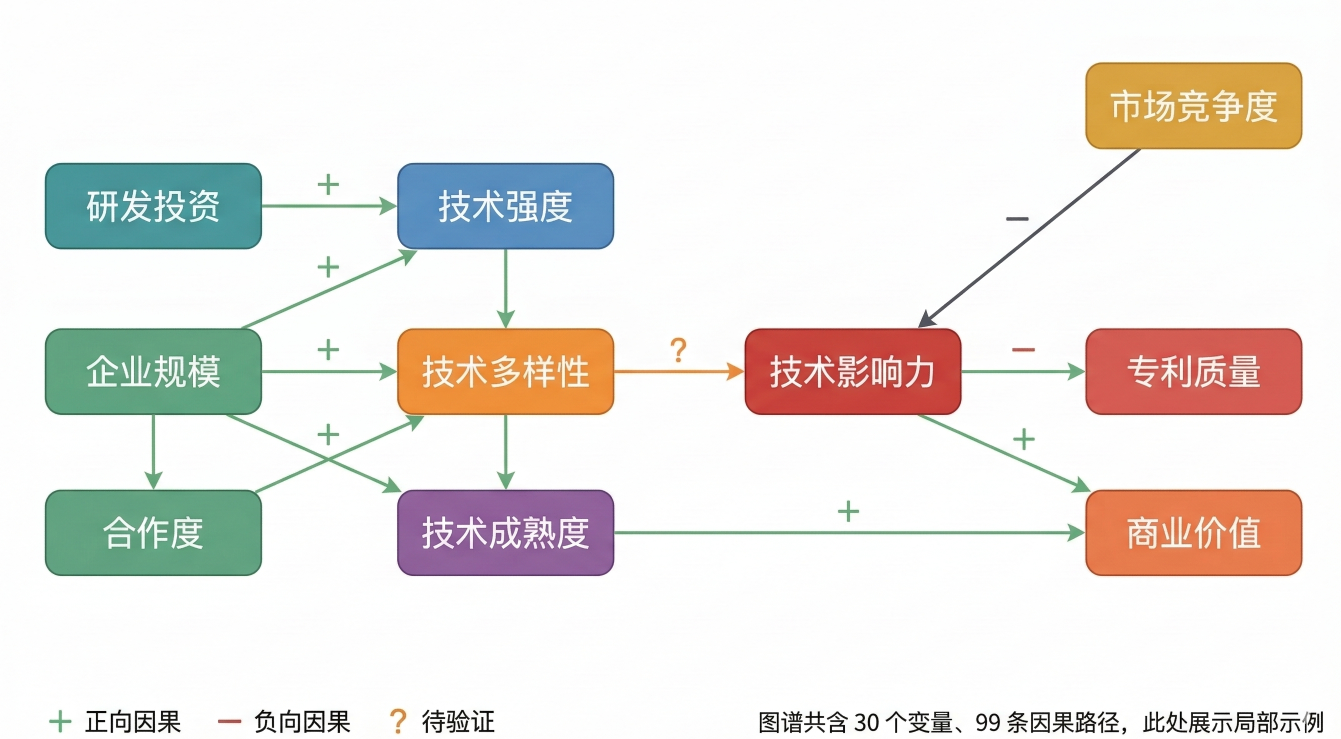
\includegraphics[width=0.95\textwidth]{figures/new_img/图4-3.png}
\caption{因果图谱局部示例}
\label{fig:4-3}
\end{figure}

变量涵盖技术强度、企业规模、研发投资、技术多样性、技术影响力、商业价值等维度。系统在运行时会根据用户研究目标在因果图中检索以目标变量为终点或起点的局部结构，并结合第三章提出的 6 种假设生成策略，对这些结构进行系统性枚举。

图谱提供 6 种假设生成策略模板：

\begin{table}[htbp]
\centering
\caption{因果图谱假设生成策略}
\label{tab:causal-strategies}
\renewcommand{\arraystretch}{1.3} % 适当增加行间距，提升长文本可读性
\begin{tabular}{@{}llp{6cm}@{}} % 根据内容长度调整列宽比例
\toprule
策略 & 核心思路 & 示例 \\ \midrule
理论迁移 & 将已验证理论应用到新场景 & 将“研发投资 $\rightarrow$ 技术产出”路径迁移至专利数据 \\
路径探索 & 发现文献中未充分研究的因果路径 & 探索“技术多样性 $\rightarrow$ 商业价值”的间接路径 \\
边界条件 & 为已知关系寻找调节变量 & 企业规模是否调节“技术多样性”与“影响力”的关系 \\
中介机制 & 揭示 $X \rightarrow M \rightarrow Y$ 的中介效应 & 技术多样性是否通过“技术成熟度”中介影响商业价值 \\
反事实推理 & 生成反直觉假设 & 技术多样性高的专利影响力反而更低？ \\
交互效应 & 探索多变量联合作用 & 研发投资与技术多样性的交互项是否显著 \\ \bottomrule
\end{tabular}
\end{table}

方法图谱包含 86 种以上的分析方法，按两个维度组织：一是变量测量方法（variable\_measurement\_methods），为每个变量 ID 提供推荐的量化方式；二是统计分析方法（statistical\_analysis\_methods），按类型分为回归分析（regression）、中介分析（mediation）、调节分析（moderation）。在工程实现上，两类知识均以可查询的 JSON 结构存储，Strategist 与 Methodologist 可通过变量 ID 和假设类型进行检索与匹配。

方法匹配逻辑：根据假设类型自动推荐适配的分析方法。例如，中介效应假设自动匹配 Bootstrap 中介检验方法；调节效应假设自动匹配层次回归方法。方法匹配示例如图 4-4 所示。通过这种显式映射，系统可以避免出现"用不恰当方法检验特定假设类型"的情况，并在不同运行之间保持方法选择的一致性。

% 图4-4
\begin{figure}[H]
\centering
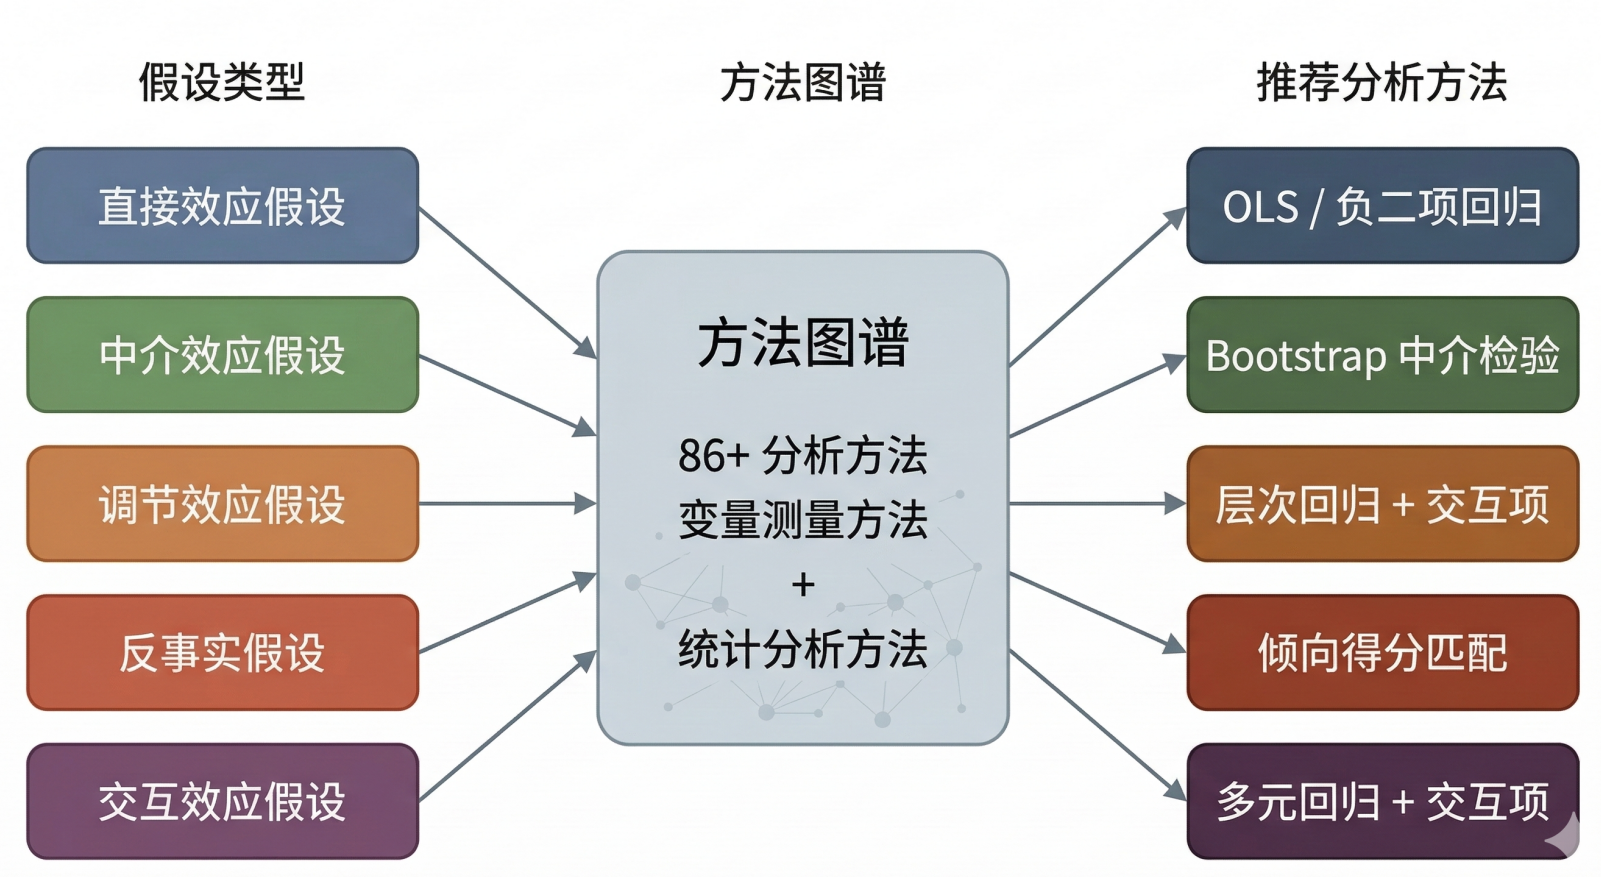
\includegraphics[width=0.95\textwidth]{figures/new_img/图4-4.png}
\caption{方法匹配示例图}
\label{fig:4-4}
\end{figure}

在 Strategist 中，双图谱的使用顺序为：先由因果图谱生成候选假设（确定"研究什么"），再由方法图谱匹配执行方法（确定"怎么做"）。该顺序保证先确定理论合理的研究方向，再确定技术可执行的实现路径，避免出现"先选方法再寻找问题"或"理论合理但工程上难以实现"的方案。此外，双图谱的查询结果会被写入蓝图节点的元数据中，便于 Reviewer 在事后审查某一任务是否真正对应了既有研究范式。

\subsubsection{分析蓝图生成与执行闭环}

\paragraph{DAG 蓝图结构}

Strategist 输出的蓝图为有向无环图（DAG），每个节点代表一个分析任务，是连接"高层研究目标"与"底层可执行代码"之间的核心中间表示。任务节点包含以下字段：

\begin{lstlisting}[basicstyle=\ttfamily\small,frame=single,breaklines=true]
{
"task_id": "task_1",
"task_type": "hypothesis_test",
"question": "技术跨界度对技术影响力是否有负向影响？",
"description": "在H04L9/40子群中进行多元回归...",
"input_variables": [],
"output_variables": ["result_1"],
"dependencies": [],
"implementation_config": {
"data_source": "data/new_data.XLSX",
"sheet_name": "sheet1",
"columns_to_load": ["IPC分类号", "被引用专利数量", "授权日"],
"parameters": {
"core_ipc": "H04L9/40",
"control_vars": ["patent_age", "legal_status_dummies"]
},
"output_format": "json",
"output_file": "outputs/task_1_result.json"
}
}
\end{lstlisting}

节点间通过 \texttt{dependencies} 字段和 \texttt{input\_variables}/\texttt{output\_variables} 字段建立依赖关系，确保任务按正确顺序执行。DAG 结构还支持在出现执行失败时，仅重跑受影响的子图，而无需重复整个流程。

Methodologist 将蓝图节点进一步转化为技术规格，包括函数签名、输入契约、变量约束、参数说明与预期输出类型。该步骤的作用是在 Strategist 的高层规划和 CodingAgent 的底层执行之间建立精确的"合同"。在实现上，Methodologist 会对蓝图中常见的不确定项（如列名模糊、参数范围不清晰）进行补全或显式标注，避免这些模糊性直接传递到代码生成阶段。

CodingAgent 基于技术规格自动生成并执行 Python 代码，执行与纠错流程如图 4-5 所示。系统为每个任务维护独立的日志与输出文件夹，记录原始代码、标准输出、错误栈信息和修复历史，便于后续复盘与人工审查。

% 图4-5
\begin{figure}[H]
\centering
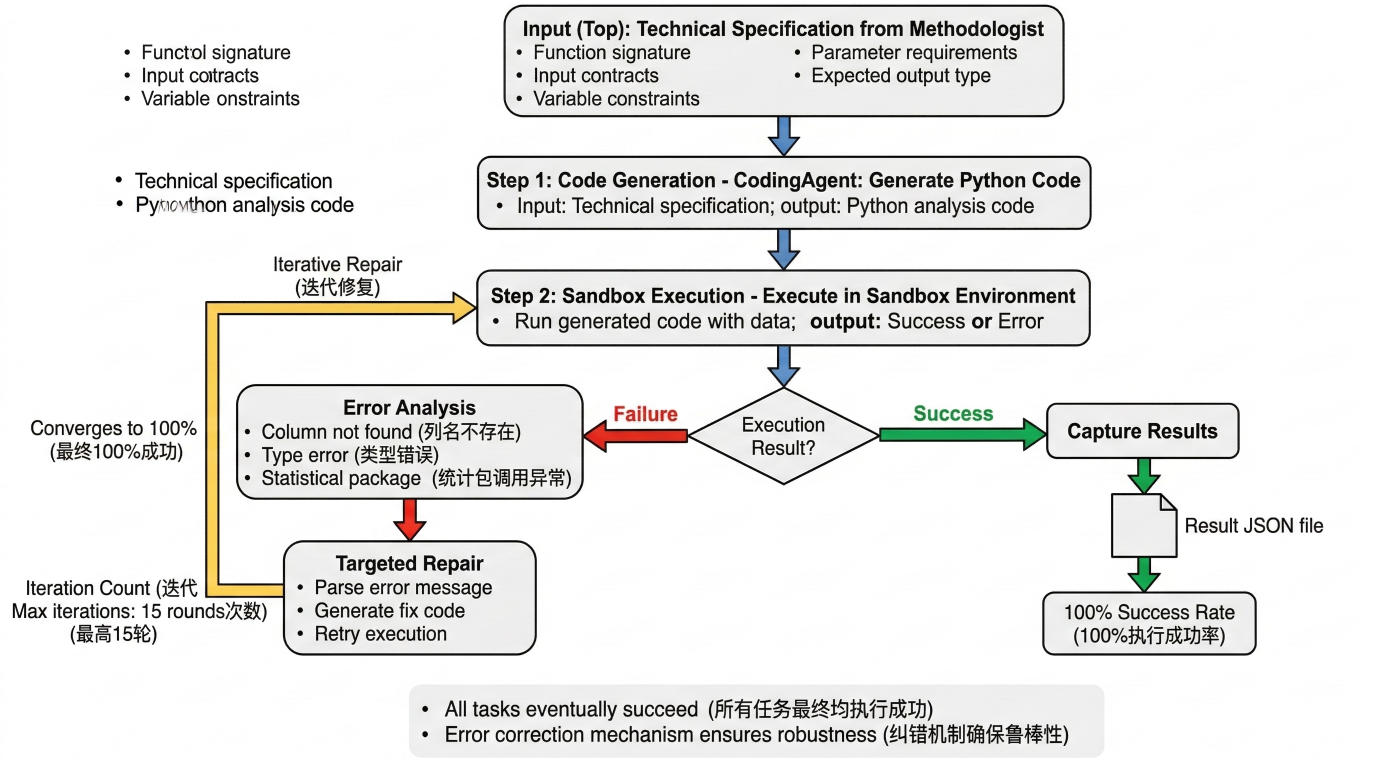
\includegraphics[width=0.95\textwidth]{figures/new_img/图4-5.png}
\caption{执行与纠错流程图}
\label{fig:4-5}
\end{figure}

若执行失败（如缺列、类型错误、统计包调用异常），系统根据错误信息触发定向修复，最多迭代 15 轮。在实验中，所有任务最终均执行成功（成功率 100\%），说明该纠错机制具有足够的容错能力。

Reviewer 对执行结果进行两个维度的评审：结构完整性检查（输出是否包含预期字段）和语义有效性评估（结论是否回答了研究问题）。评审结果用于最终报告生成，并为差距分析和第二轮规划提供输入，相当于在流水线末端增加一道"LLM-as-judge"式的质量闸门。

\subsubsection{两轮迭代机制}

两轮机制通过 \texttt{round} 与 \texttt{previous\_results} 传递上下文，第二轮蓝图由 \texttt{\_generate\_refined\_blueprint()} 方法生成。与第三章的方法论设计相呼应，这里给出了在工程实现层面如何编码"探索—验证"闭环的具体做法。

\paragraph{第二轮蓝图生成流程}

第二轮 Prompt 包含三个额外输入：

\begin{enumerate}
\item 第一轮各任务的执行结果摘要（关键发现、统计量、结论）
\item 差距分析：评估第一轮"已回答"和"未充分回答"的问题边界
\item 深化策略：补充控制变量、增加交互项检验、引入非线性模型
\end{enumerate}

\begin{algorithm}[H]
\caption{两轮规划流程}
\KwIn{用户研究目标 goal, 数据集 data}
\KwOut{两轮分析结果 final\_results}

\tcp{第一轮：探索性分析}
insights $\leftarrow$ GenerateDataInsights(data, goal)\;
blueprint\_1 $\leftarrow$ Strategist(goal, data, insights, round=1)\;
results\_1 $\leftarrow$ Execute(blueprint\_1) \tcp{Methodologist $\rightarrow$ CodingAgent $\rightarrow$ Reviewer}
\tcp{第二轮：验证性分析}
gap $\leftarrow$ AnalyzeGap(results\_1, goal, insights)\;
blueprint\_2 $\leftarrow$ Strategist(goal, data, insights, round=2, previous\_results=results\_1, gap=gap)\;
results\_2 $\leftarrow$ Execute(blueprint\_2)\;
final\_results $\leftarrow$ Merge(results\_1, results\_2)\;
\Return{final\_results}\;
\end{algorithm}

迭代效果与单轮流程相比，两轮机制将系统行为从"一次性生成"改为"反馈驱动生成"。实验中，第二轮常见的新增操作包括：负二项回归替代 OLS（非线性建模）、BERT 主题建模（文本挖掘）、IPC 共现网络特征工程（图结构利用）、交互项检验（机制验证）。这些操作将分析从效应发现提升至机制解释层次，也为系统在报告中给出"第一轮结论在何种条件下仍然成立"提供了证据基础。

\subsection{本章小结}

本章围绕“把第三章的系统设计落到可运行原型”这一目标，给出了系统核心模块的实现细节与关键工程策略，形成了一套从数据预览到方案生成、从自动执行到结果复核的闭环实现路径。

在数据感知层，DataPreview 通过列语义识别、类型画像与跨列统计（相关、分组对比、时间趋势）将“表格事实”压缩为结构化证据；同时结合分层抽样补充专利摘要样本，使规划阶段能够在有限上下文内把握技术内容分布。GraphPreview 作为补充维度，通过自动构图与分层图算法策略提取“关系结构事实”，在中小规模图上输出社区、中心性与连通性等指标，在大规模图上自动降级以控制复杂度，从工程上兼顾了信息密度与响应时间。

在洞察到蓝图的转换层，实现了数据洞察生成机制：通过约束性 Prompt 将统计信号、图结构特征与内容样本综合为可检验洞察，并要求洞察显式引用输入中的具体数字、指明数据列与分析方法，从而抑制空泛表述和常识性结论。该机制使系统的规划不再是“问题语义驱动”，而是以“证据驱动”为主线，为后续 DAG 蓝图生成提供了稳定的起点与边界。

在知识约束层，双知识图谱在工程上被实现为可查询的结构资源：因果图谱用于收缩与组织假设空间，方法图谱用于约束方法选择与变量测量路径。通过“先假设后方法”的协同调用方式，系统能够在保持可执行性的前提下，将领域共识嵌入到蓝图元数据中，并支持在不同任务之间复用一致的约束逻辑，提升方案的可比性与可复核性。

在执行与迭代层，本章实现了“规划—规格—执行—评审”的闭环流水线，并在其上叠加两轮迭代机制。第一轮用于快速建立主效应与关键结构信号，差距分析对未覆盖方向与薄弱证据进行诊断，第二轮则围绕证据缺口引入控制变量、非线性建模、交互效应或机制检验，推动分析从“效应发现”提升到“机制解释与边界条件”的层次。由于蓝图、技术规格、代码与结果均以结构化文件持久化保存，系统具备较好的追踪性与可复现性，也为后续开展对比实验与消融评估提供了可靠的工程基座。

本章所实现的 DataPreview/GraphPreview、数据洞察生成、双知识图谱与两轮迭代机制共同构成可复核、可迭代的自动分析原型，为第五章的实验与评估提供了可操作的技术基础与过程证据链。
